%
%  Vorlage/Template fuer #Proseminar
%
%  Created by Claudia Pittel und Yunus Erdemir in 2018, updated in 2021.
%  Copyright (c) 2021 . All rights reserved.
%
\documentclass[12pt,toc=bib,toc=listof]{scrreprt}
\usepackage[ngerman]{babel} 
\usepackage[utf8]{inputenc}
\usepackage[T1]{fontenc}
% Standardschriftart Latin Modern
\usepackage[scaled]{helvet}
\renewcommand\familydefault{\sfdefault}
% Arial, so in etwa
%\usepackage{newtxmath,newtxtext}
%Times New Roman, so in etwa
% Zitate durchgehend nummerieren
\usepackage{chngcntr}
\counterwithout{footnote}{chapter}
%Zeilenabstand
\usepackage{setspace}
\linespread{1.3}

% DIN-A-4, Ränder (oben, links, rechts, unten), Abstand Kopfzeile und Text
\usepackage{geometry}
\geometry{a4paper, top=25mm, left=30mm, right=20mm, bottom=25mm, headsep=12mm}

\usepackage[backend=bibtex, style=authortitle-ibid, url=false, isbn=false, doi=false]{biblatex}
\addbibresource{literature.bib}

\usepackage{hyperref}
\hypersetup{
  ,colorlinks=true
  ,linkcolor=blue
  ,citecolor=blue
  ,filecolor=blue
  ,urlcolor=blue
  }

%%%%%%%%%%%%%%%%%%%%%%%%%%%%%%%%%%%%% % (fold)
% Vom Studierenden zu aendernde Werte
\newcommand{\topic}{XaaS - Anything as a Service}

\newcommand{\studentnameA}{Suphi Pembe}
\newcommand{\studentidA}{207617}
\newcommand{\studentpartA}{SEITEN oder KAPITEL VON BIS 1}

\newcommand{\studentnameB}{Andreas Würzer}
\newcommand{\studentidB}{207258}
\newcommand{\studentpartB}{SEITEN oder KAPITEL VON BIS 2}

\newcommand{\studentnameC}{Christian Nguyen}
\newcommand{\studentidC}{207613}
\newcommand{\studentpartC}{SEITEN oder KAPITEL VON BIS 3}

\newcommand{\semester}{Sommersemester 2022}
%
%%%%%%%%%%%%%%%%%%%%%%%%%%%%%%%%%%%%% % (end)

\usepackage{ifpdf}
\ifpdf
\usepackage[pdftex]{graphicx}
\else
\usepackage{graphicx}
\fi

\usepackage[headsepline,footsepline]{scrlayer-scrpage}
\pagestyle{scrheadings}
\clearpairofpagestyles
\ihead{Proseminar: \topic}
\ofoot{Seite \pagemark}
\renewcommand*{\chapterpagestyle}{scrheadings}
\renewcommand*{\chapterheadstartvskip}{}

% Logo
\titlehead{\flushright
\includegraphics[scale=0.5]{HHN_Logo_D_oS_RGB_300.png}}
\subject{Proseminar (282136)}
\title{\topic}
\author{\studentnameA { ({\studentidA)}}, \\ \studentnameB { ({\studentidB)}}, \\ \studentnameC { ({\studentidC)}} }
\date {\semester}
%% Datum nie auf einen festen Wert setzen
\publishers{Vorgelegt bei Claudia Pittel}

%\pagestyle{headings}

% Zähler für Römische Nummerierung
\newcounter{savepage}

\begin{document}
\pagenumbering{roman} 
\selectlanguage{ngerman}
\sffamily
% serifenlose Schriftfamilie
\maketitle

\addchap{Management Summary} % (fold)
\label{sec:management_summary}

Hier sollte ziemlich genau bzw. maximal 1 Seite Text stehen (ziemlich genau  bedeutet, man sollte so nah wie möglich an 1 Seite herankommen).
Text für Test commit haha

% chapter management_summary (end)

\tableofcontents

\addchap{Abkürzungsverzeichnis} % (fold)
\label{sec:abkuerzungsverzeichnis}

\begin{description}
\item[GPU] Graphics-Processing-Unit oder Grafikkarte
\item[HPC] High-Performance-Computing
\item[RAID] redundant array of independent disk
\end{description}

% chapter abkuerzungsverzeichnis (end)

\listoffigures
\listoftables

% \onehalfspacing

\newpage
% Zähler speichern
\setcounter{savepage}{\arabic{page}}
\pagenumbering{arabic}

\chapter{Einleitung} % (fold)
\label{sec:einleitung}

Einleitungstext mit Motivation, Ziel der Arbeit (d.h. Erläuterung der Forschungsfrage) und Beschreibung der Vorgehensweise bzw. Aufbau der Arbeit\footcite [vgl.] [S. 38]{Th17}

\section{Motivation} % (fold)
\label{sec:motivation}
%%%% Version 1 %%%%%%%%
Durch den aktuell anhaltende Halbleitermangel besteht ein Engpass an Ressourcen von die meisten Wirtschaftszweige betroffen sind.
Einer dieser Wirtschaftszweige ist die Produktion von GPUs (graphics processing unit. Diese werden für diverse Anwendung von Computern verwendet, im betrieblichen wie auch im privaten Bereich.
Primär in dieser Arbeit werden die Bereiche High-Performance-Computing (HPC) und Gaming haben.
Beide diese Bereiche benötigen GPU-Rechenleistung, welche im konventionell von einer lokal verbauten GPU zur Verfügung gestellt wird. 
Als Langfristige Lösung soll analysiert werden ob es möglich ist durch zentrale Services, welche GPU as a Service anbieten. 
Durch die zentralen Ressourcenteilung dem Mangel entgegenzuwirken mit einer alternative für den Bedarf zu schaffen.

% section motivation (end)

\section{Ziel der Arbeit} % (fold)
\label{sec:ziel_der_arbeit}

\ldots

% section ziel_der_arbeit (end)

\section{Vorgehensweise} % (fold)
\label{sec:vorgehensweise}

\ldots

% section vorgehensweise (end)
% chapter einleitung (end)

\chapter{Anything as a Service - Cloud Computing} % (fold)
\label{sec:Anything as a Service - Cloud Computing}

Zwischen den Gliederungspunkten sollten jeweils kurze Überleitungssätze stehen, damit man weiß, um was es inhaltlich in den folgenden Unterkapiteln geht.\footcite [Vgl.] []{GPL}

% chapter ersteskapitel (end)

\section{Definition} % (fold)
\label{sec:Definition}

Bei den Gliederungspunkten immer auf eine Ausgewogenheit achten, damit eine gleichmäßige Gliederung gefördert werden kann. Sofern Abbildungen (wie Abbildung 1: Beispielbild) verwendet werden, müssen diese auch inhaltlich im Text erwähnt und erläutert werden, sowie ein Abbildungsverzeichnis erstellt werden.\footcite [Vgl.] [] {hhnwin}

% section unterkapitel1 (end)

\section{Typische Servicemodelle} % (fold)
\label{sec:Typische Servicemodelle}

Untergliederungen nur in der Mehrzahl erstellen, d.h. nie 1 Unterkapitel alleine stehen lassen.
In gleicher Art und Weise wie Abbildungen dargestellt und beschriftet werden, verhält es sich mit Tabellen.

% section unterkapitel1 (end)

\subsection{IaaS: Infrastructure as a Service}
\label{sec:IaaS: Infrastructure as a Service}

Inhalt

\subsection{SaaS: Software as a Service}
\label{sec:SaaS: Software as a Service}

Inhalt

\subsection{PaaS: Plattform as a Service}
\label{sec:PaaS: Plattform as a Service}


\section{Vor- und Nachteile}
\label{Vor- und Nachteile}

\chapter{Knappheit von Grafikkarten} % (fold)
\label{sec:Knappheit von Grafikkarten}

Die Knappheit von Grafikkarten hat den
aktuellen Markt durch neue Branchen die GPU-Leistung nutzen nachhaltig verändert.
Diese Knappheit entsteht nicht nur durch den Mangel des Rohstoffes, sondern auch durch die 
Weiterentwicklung von verwendeten Computern in allen Einsatzgebieten.\footcite [Vgl.] []{Voas.2021}
\\
%\begin{figure}[h]
%  \centering
%  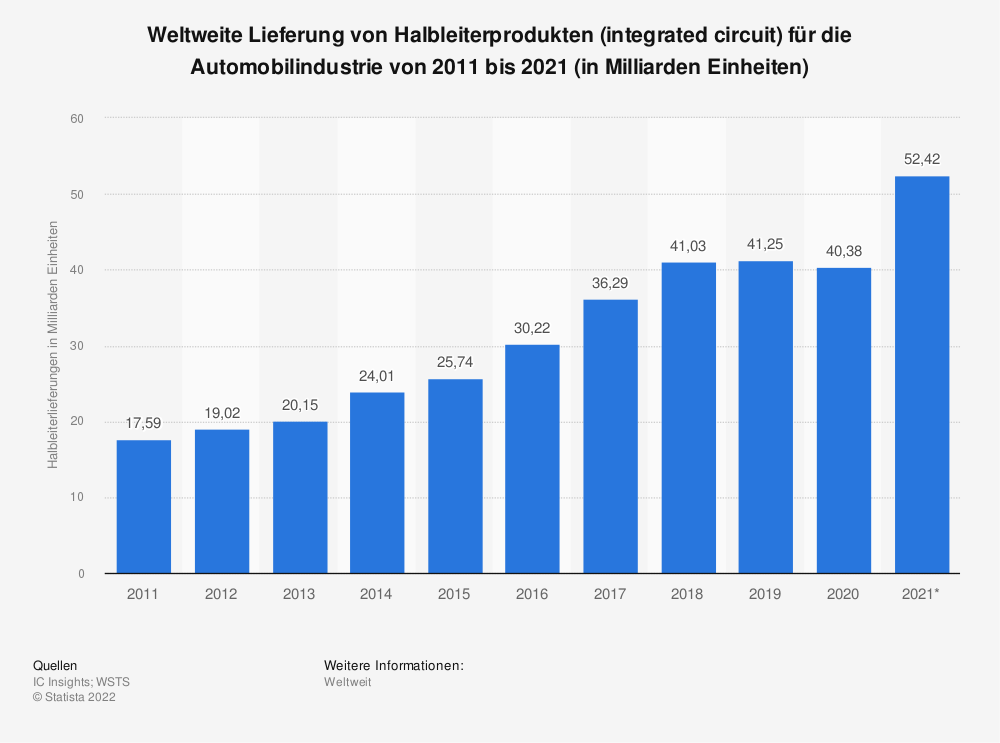
\includegraphics[scale=0.35]{Abbildungen/Martin_Kords_1.png} % 0,9 ursprünglich, auf Seite anpassen
%  \caption[]{Weltweite Lieferung von Halbleiterprodukten für die Automobilindustrie von 2011 bis 2021}
%\end{figure}
\\
Im Vergleich zu 2011 wurden für die Automobilindustrie im Jahr 2021 fast drei mal so viele
Halbleiter geliefert. Ebenfalls mit der Weiterentwicklung von Internet of Things Produkten wird in
Zukunft der Bedarf an Halbleitern weiter steigen.\footcite [Vgl.] []{Bill_McClean} \footcite [Vgl.] []{Voas.2021} 
%Quelle https://www.icinsights.com/news/bulletins/The-Real-Reason-Behind-The-Automotive-Industry-IC-ShortageA-StepFunction-Surge-In-Demand/
\\In diesem Kapitel soll die Preisentwicklung von GPUs betrachtet werden, dabei wird 
ein Zusammenhang geschaffen mit den Ursachen die diese Preisentwicklung 
verursacht haben.
\\

\section{Preisentwicklung}
\label{sec:Preisentwicklung}

Die rapide steigende Preisentwicklung von GPUs ist auf zwei Kernfaktoren reduzierbar.\\
- Größerer Bedarf an GPUs und Halbleitern, dem Kernbestandteil von GPUs\\ %Beispiel aufgezeigt
- Mangelnde Kapazitäten zur Produktion von Halbleitern\\
Der Bedarf an Halbleitern und GPUs ist konstant im Anstieg. Besonders durch die Corona Pandemie,
hat sich im Vergleich zu 2019 im Jahr 2020 ein Umsatzanstieg von 5,4\% aufgezeigt.\footcite [Vgl.] []{Voas.2021}
%\begin{figure}[h]
%  \centering
%  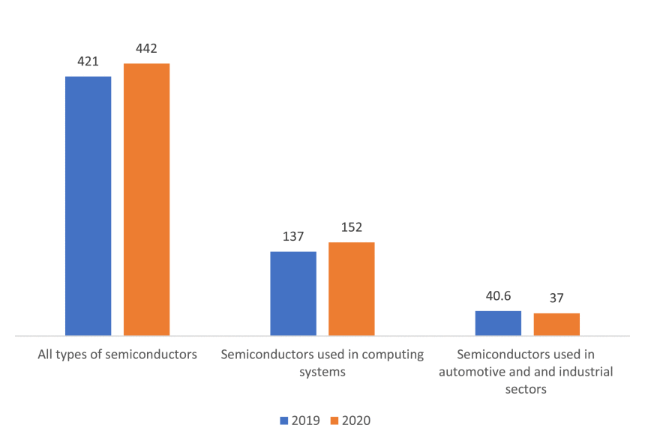
\includegraphics[scale=0.9]{Abbildungen/voas1.png} % 0,9 ursprünglich, auf Seite anpassen
%  \caption[]{Worldwide semiconductor revenues in 2019 and 2020 (dollar, billions)}
%\end{figure}
\\Wie in Abbildung 3.2 zu sehen ist der Umsatzanstieg größtenteils durch Erlöse von Computersystemen entstanden.
Im Vergleich dazu sind Umsätze, die durch Abnehmer in der Automobilbranche entstanden sind gesunken.
Das lässt sich auf den steigenden Bedarf an Computersystemen zurückführen. Während der Pandemie mussten
viele Menschen Home-Schooling und Home-Office aneignen, um weiter den Alltagsbetrieb ausführen zu können.
Ein Nebenläufiger Effekt ist damit, dass durch die Digitalisierung weniger Mobilität benötigt wird.
Damit lässt sich der reduzierte Bedarf an Halbleitern erklären. Dennoch ist damit insgesamt der Bedarf an 
Halbleiter gestiegen.\footcite [Vgl.] []{Voas.2021}
\\\\ Der steigende Bedarf allein ist aber wie angeführt nicht der einzige Faktor. Die Produktion 
von Halbleitern stagniert. Das lässt sich auf verschiedene Ursachen zurückführen. Da die meisten 
Halbleiter in asiatischen Ländern produziert werden und diese den eigenen Bedarf zuerst decken, ist 
für den Export weniger Verfügbar. Ebenfalls haben sin in den letzten Jahren Naturdesaster ereignet die
Ebenfalls durch z.B. Dürre die Produktion Lahmgelegt haben.\footcite [Vgl.] []{Voas.2021}
\\
Durch mangelnde Produktion und steigender Bedarf hat sich nun ein sehr hoher Marktpreis entwickelt. 
Um diesem Entgegenzuwirken ist nicht nur Ressourcenverfügbarkeit zu schaffen, sondern auch eine effizientere Methode
die Ressourcen zu nutzen.

\section{Ursache Halbleitermangel und KryptoMining}
\label{sec:Ursache Halbleitermangel und KryptoMining}

Um den Halbleitermangel besser zu verstehen, sollten eine neue Branche die primär GPU-Leistung 
nutzt thematisiert werden. Seit dem Jahr 2021 haben Kryptowährungen ein mehr als fünffaches Investitionsvolumen
im Vergleich zum Vorjahr.\footcite [] [] {Statista_Research_1}
\\Um den Zusammenhang zu erläutern, Kryptowährungen validieren Ihre Transaktionen durch die Nutzung der 
Blockchain-Technologie. Bei diesem Validierungsprozess werden neue Datenblöcke in einer Datenbank gespeichert und von anderen
Nutzern überprüft durch eine Prüfsumme die dabei gebildet werden können muss. Um diese Prüfsumme berechnen zu können
Nutzen sogenannte "Krypto-Miner" primär GPU-Leistung.\footcite [Vgl.] [S.259-273] {Arslanian.2022}
\\Da große Investitionen für das Kryptomining getätigt werden hat sich ein neuer Markt mit einer großen Nachfrage gebildet, der
GPUs benötigt.
\\ \\
%Ein Ende in Sicht?
%https://www.gartner.com/en/newsroom/press-releases/2021-05-12-gartner-says-global-chip-shortage-expected-to-persist-until-second-quarter-of-2022
%
Allerdings gibt es Faktengestütze Prognosen, welche behaupten das der Halbleitermangel nicht zu lange anhalten wird. 
Nach Gartner war die Prognose auf das zweite Quartal 2022 geschätzt, auch wenn dies nicht im vollen Umfang eingetreten ist sind 
die Argumente für die weitere Zukunft nicht irrelevant.\\
Angeführt wird das durch den Halbleitermangel nun die Lieferkette enger überwacht wird.
Daraus resultierend wird mehr transparenz und vorinverstionen um die Lieferung garantieren zu können. 
Ebenfalls möchte man auch die Abnahme von mehreren Lieferanten bevorzugen, anstatt von einem Lieferanten abhängig zu sein.
Diese Faktoren sollen Langfristig Sicherheit in der Lieferkette schaffen. \footcite [Vgl.] [] {Gartner.2021}

\chapter{Gaming as a Service}
\label{sec: Gaming as a Service}

Cloud Computing umfasst die Bereitstellung von Rechenleistung und Anwendungen als Dienst über das Internet und soll daher mit Gaming-as-a-Service als Beispiel vertieft werden. Neben der Funktionsweise, werden auch die aktuell verfügbaren Angebote verglichen und damit dem Kauf eines eigenen Computers gegenübergestellt.

\section{Funktionsweise}
\label{sec:Funktionsweise}

Die Ausführung der Spiele, einschließlich der Spielelogik und Wiedergabe der Szenen findet innerhalb der Cloud bzw. Server statt. In Verbindung steht das Gerät des Endnutzers, oder auch Thin-Client genannt. Dieser empfängt die komprimiert gestreamten Audio- und Videosignale über das Internet und gibt sie auf dem Thin-Client wieder. Bei eingehenden Befehlen des Endnutzern, werden diese erfasst und an die Cloud übertragen. Durch die Leistung des Netzwerks zwischen dem Client und der Cloud sind die Prozesse eingeschränkt.

\section{Anbietervergleich}
\label{sec:Anbietervergleich}

Inhalt

\subsection{Voraussetzung}
\label{sec:Vorraussetzung}

Inhalt

\subsection{Angebot}
\label{sec:Angebot}

Inhalt

\subsection{Preis}
\label{sec:Preis}

Inhalt

\section{Hardwarevorraussetzung um Usability zu gewährleisten}
\label{sec:Hardwarevorraussetzung um Usability zu gewährleisten}

Inhalt

\chapter{GPU as a Service}
\label{sec:GPU as a Service}

Außerhalb von Gaming as a Service gibt es weitere Service 
Möglichkeiten die ebenfalls GPU as a Service beanspruchen bzw. inkludieren. Wachsende Märkte dafür sind
das rendern von 3D-Modellen und animierten Videos, 
wie auch deep learning model training für KIs. 
\\Im folgenden Kapitel wird erläutert werden wie GPU as a Service Anbieter Ihren Service 
realisieren können und Qualität schaffen mit verschiedenen Methoden. 
Wie auch die Einsatzgebiete feststellen und identifizieren in 
welchen von diesen Einsatzgebiete sich eine Cloud-Lösung eignet.

\section{Funktionsweise}
\label{sec: Funktionsweise}

Bei der Dienstleistung Inanspruchnahme werden von die von einem geforderten
Prozesse, wie z.B. das rendern von 3D-Modellen, durch die Rechenleistung des 
Anbieters verarbeitet. Im Gegensatz zu der Privatnutzung bei der nur eine GPU genutzt wird, 
verwenden GPU a as Service Anbieter mehrere GPUs. 
Allerdings da GPUs nur als Co-Prozessoren in solchen Systemen genutzt werden, 
können diese nicht eigenständig betrieben werden sondern benötigen einen zentrales 
Betriebssystem, auch Kernel bezeichnet. Üblicherweise wird das skalierbar angewendet mit einer
Vielzahl an Kernels, welche eine Vielzahl an GPUs besitzen.\footcite [Vgl.] [] {Wang.2017}
\\% auskommentiert für Textmessen
%\begin{figure}[h]
% \centering
%  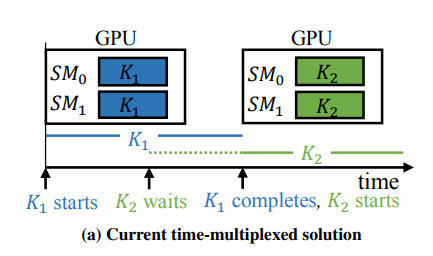
\includegraphics[scale=1.4]{Abbildungen/wang1.png} 
%  \caption[]{Current time-multiplexed solution}
%\end{figure}
\\%
Es gibt verschiedene Methoden diese Prozesse darauf zu verarbeiten. Eine Methode davon 
ist das Zeit-Multiplexverfahren. Bei diesem Verfahren werden mehrere Prozesse auf die Kernels
sequenziell aufgeteilt und verarbeitet, wie in Abbildung 5.1 zu sehen. Dieses Methode 
hat keinen direkten Mehrwert in Bezug zur Verarbeitungseffizienz, allerdings verhindert 
sie das Prozesse Kernels unnötig blockieren. \footcite [Vgl.] [] {Wang.2017}
\\ \\
%Andere Methode erklären aus der selben Quelle
Ein anderer Ansatz um Konstanz zu schaffen ist das das man die Kernels über Software zu einen Kernel fusioniert. 
Das ist vergleichbar mit dem für Festplatten verwendete "redundant array of independent disk"-System auch abgekürzt genannt RAID, 
welches gängiger bekannt ist. Durch das fusionieren der Kernels über die Software kann eine 
konstante Leistung gewährleistet werden.
Ebenfalls auch eine fairness zwischen allen Leistungsabnehmern, da es keine Situation geben kann einen schlechten Kernel erwischt zu haben.\footcite [Vgl.] [] {Wang.2017}
\\ \\
Eine quasi gegenteilige Methode die Kernels in verschiedene Partitionen aufzuteilen, anstatt Sie zu fusionieren.
Wiedermal vergleichbar wie man auch mit Festplatten umgehen kann. Die Leistung des Kernel wird 
in verschiedene Partitionen aufgeteilt. Diese können dann je nach Monetarisierungsmodel 
vermietet werden für einen Zeitraum oder auf einer Bedarfsbasis. Daraus besteht der Vorteil, 
dass Nutzer des Services Ihren Bedarf selbst definieren können und garantiert diese Leistung 
in Anspruch nehmen können. \footcite [Vgl.] [] {Wang.2017}

\section{Einsatzgebiete}
\label{sec: Einsatzgebiete}

%Wachsende Märkte dafür sind
%das rendern von 3D-Modellen und animierten Videos, 
%wie auch deep learning model training für KIs.

Die Einsatzgebiete sind weitreichend und können auf zwei Bedarfsmethoden eingeteilt werden.
Einmal in Schüben, in denen ein festes Ziel und der Aufwand definiert wird, welcher der Prozess erreichen soll.
Beispiele dafür sind rendern von 3D-Modellen und animierten Videos.
\\ 
Um dieses Beispiele auszuführen, wenn ein 3D-Modell dargestellt wird. Das 3D-Modell besteht aus Matrixoperationen die von GPUs 
in der Regel berechnet werden. Meist mit dem Ziel diese realitätsgeträu und logisch in einer Umgebung darzustellen.
Dieses Beispiel lässt erweitern auf animierte Videos, bei diesen dann eine veränderte Version des Vorgängermodells oder ein 
vollkommen anderes Modell für jedes Bild das gezeigt wird. \footcite [Vgl.] [] {Loop.2006}
\\ \\
Ebenso ist es möglich, dass optinal mit einem Ziel aber unbekannten Aufwand, so ein Prozess ausgeführt wird. 
In diesem Fall wird eine konstante Rechenleistung benötigt wird.
Beispiele dafür sind deep learning modelle für KIs oder Gaming as a Service.
\\
Um hier Ebenfalls ein Beispiel anzuführen, wenn Gaming as a Service Dienste in Anspruch genommen.
Bei diesem Service ist kein Ziel festgelegt, da auch nicht ein konkreter Prozess vorgegeben wird.
Anhand der Eingaben des Nutzers variert die benötige Visualsierung und Spielelogik. Da die Eingaben 
nicht vorher konkret bekannt sind, wird besteht ein konstanter Bedarf an Rechenleistung um auf die Eingaben 
reagieren zu können. Die Rechenleistung wird benötigt bis der Nutzer das Spiel beendet. \footcite [Vgl.] [] {Lattuada.2022} \footcite [Vgl.] [] {Wang.2017} \footcite [Vgl.] [] {Loop.2006}
%Schlussfolgerung aus eigenem Wissen und den Papers

\section{Vergleich eigene GPU und GPU in der Cloud}
\label{sec:Vergleich eigene GPU und GPU in der Cloud}

Nach dem angeführten Informationen lässt sich folgendes feststellen. 
Der Bedarf an GPU Rechenleistung ist im konstanten Wachstum für verschiedene Märkte. Die GPU as a Service Anbieter 
können Ihre Systeme entsprechend dem Monetarisierungsmodel und dem Leistungsprioritäten aufstellen. Dabei sind das 
keine neue Methoden und vergleichbar mit der Massenspeicherverwaltung. Je nach geplanter Nutzung werden GPUs 
entweder in Schüben oder Konstant Rechenleistung abverlangt.\\ \\
Nach unserem ermessen ist besonders die Entscheidung zwischen der eigenen GPU oder GPU as a Service abhängig der 
benötigten Rechenleistung und der Verfügbarkeit. In der Annahme das der Dienstleister des GPU as a Serive permanent 
Verfügbar ist. Sollten für Prozesse welche in Schüben erfolgen GPU as a Service ein attraktives Angebot sein, da 
diese mit der großen Rechenleistung diese Prozesse in kurzer Zeit abgeschlossen werden können.\\ \\
Eine eigene GPU ist attraktiv eher im Fall von Konstant benötigter Rechenleistung. Wenn eine Verfügbare GPU in der Lage 
die benötigte Rechenleistung zu erbringen. Andernfalls ist GPU as a Service ebenfalls eine Lösung, besonders in Zeiten 
in denen die Preise von GPUs mit dem Halbleitermangel gestigen sind.\\

\chapter{Marktvorhersage}
\label{sec:Marktvorhersage}

Inhalt

\chapter{Fazit und Ausblick} % (fold)
\label{sec:fazit}

Kritische Begutachtung inklusive Zusammenfassung der Arbeit sowie eventuelle Zukunftsperspektiven zum Thema können hier im Fazit und im Ausblick eingebracht werden.\footcite [Vgl.] [] {HAN2016S30}

% chapter fazit (end)

\appendix
\newpage

\pagenumbering{roman}
% Zähler laden
\setcounter{page}{\thesavepage}

\addchap{Anhang} % (fold)
\label{sec:anhang}

Der Anhang soll den eigentlichen Hauptteil nicht ergänzen, sondern darüber hinaus weitere möglicherweise interessante Informationen liefern, die aber nicht zwangsläufig notwendig sind, um den Hauptinhalt zu verstehen

\newpage

% Quellen wird erst dargestellt sobald ein Zitat verwendet wird
\defbibheading{head}{\addchap{Quellenverzeichnis}}
\printbibliography[heading=head]

%\vspace{2cm}

%Hier müssen alle Quellenverweise zu finden sein – inklusive aller erforderlichen Angaben, alphabetisch sortiert. Eine Unterteilung in verschiedene Quellenarten ist grundsätzlich nicht notwendig, da die unterschiedlichen Quellenarten anhand der Angabe der bibliographischen Angaben zu erkennen ist. (d.h. beispielsweise keine Unterteilung zwischen „Printquellen“ und „Internetquellen“!)

\newpage

\addchap{Ehrenwörtliche Erklärung} % (fold)
\label{sec:erklaerung}

„Wir versichern, dass die vorliegende Arbeit von uns selbständig und ausschließlich unter Verwendung der angegebenen Quellen und Hilfsmittel angefertigt wurde. Alle Stellen, die wörtlich oder annähernd aus Veröffentlichungen entnommen sind, haben wir als solche kenntlich gemacht. Die Arbeit wurde bisher in gleicher oder ähnlicher Form, auch nicht in Teilen, keiner anderen Prüfungsbehörde vorgelegt und auch nicht veröffentlicht.“

\vspace{1cm}
\noindent
{\studentpartA} wurden von {\studentnameA} verfasst.
\\
{\studentpartB} wurden von {\studentnameB} verfasst.
\\
{\studentpartC} wurden von {\studentnameC} verfasst.

\vspace{3cm}
Ort, Datum \hfill Unterschrift

\vspace{2cm}
Ort, Datum \hfill Unterschrift

\vspace{2cm}
Ort, Datum \hfill Unterschrift


\end{document}
